
\chapter{Rosenbaum-Style $p$-Values for Matched Observational Studies with Unmeasured Confounding}
\chaptermark{Sensitivity Analysis in Matching}\label{sec::rosenbaum-sensitivity-analysis}


\citet{rosenbaum1987sensitivity} introduced a sensitivity analysis technique for matched observational studies. Although it works for general matched studies \citep{rosenbaum2002design}, the theory is most elegant for one-to-one matching. 
Different from Chapters \ref{chapter::evalue} and \ref{chapter::sensitivity-ACE}, Rosenbaum-type sensitivity analysis works best for matched observational studies for testing the sharp null hypothesis of no individual treatment effect.  


\section{A model for sensitivity analysis with matched data}


Consider a matched observational study, with $(i,j)$ indexing unit $j$ in pair $i$ $(i=1,\ldots, n; j=1,2)$. 
With exactly matched pairs, unit $(i, 1)$ and unit $(i, 2)$ have the same covariates $X_i$. 
Assume IID sampling, and extend Definition \ref{def::pscore} to define the propensity score as
$$
e_{ij} = \pr\{  Z_{ij} = 1\mid X_i, Y_{ij}(1), Y_{ij}(0) \} .
$$
Let $\mathbb{S}_i = \{Y_{i1}(1), Y_{i1}(0), Y_{i2}(1), Y_{i2}(0)\}$ denote the set of all potential outcomes within pair $i$. 
Conditioning on the event that $Z_{i1} + Z_{i2} = 1$, we have
\begin{eqnarray*}
\pi_{i1} &=& \pr\{ Z_{i1} = 1 \mid X_i, \mathbb{S}_i, Z_{i1} + Z_{i2} = 1 \} \\
&=& \frac{ \pr\{ Z_{i1} = 1, Z_{i2} = 0  \mid X_i, \mathbb{S}_i \} }
{ \pr\{ Z_{i1} + Z_{i2} = 1 \mid X_i, \mathbb{S}_i \} } \\
&=& \frac{ \pr\{ Z_{i1} = 1, Z_{i2} = 0  \mid X_i, \mathbb{S}_i \} }{ 
\pr\{ Z_{i1} = 1, Z_{i2} = 0 \mid X_i, \mathbb{S}_i \} + \pr\{ Z_{i1} = 0, Z_{i2} = 1 \mid X_i, \mathbb{S}_i \}
}\\
%{ \left[ \splitfrac{ \pr\{ Z_{i1} = 1, Z_{i2} = 0 \mid X_i, \mathbb{S}_i \} }
%{+\pr\{ Z_{i1} = 0, Z_{i2} = 1 \mid X_i, \mathbb{S}_i \} } \right] } \\
&=& \frac{  e_{i1} (1-e_{i2}) }{ e_{i1} (1-e_{i2}) + (1-e_{i1}) e_{i2}} 
\end{eqnarray*}
Define $o_{ij} = e_{ij} / (1 - e_{ij})$ as the odds of the treatment for unit $(i,j)$, and we have
$$
\pi_{i1}  = \frac{o_{i1}}{  o_{i1} + o_{i2} } . 
$$
Under ignorability, $e_{ij}$ is only a function of $X_i$, and therefore, $e_{i1} = e_{i2}$ and $\pi_{i1} = 1/2 $. Thus the treatment assignment mechanism conditional on covariates and potential outcomes is equivalent to that from an MPE with equal treatment and control probabilities. This is a strategy to analyze matched observational studies we discussed in Chapter \ref{sec::ideal-matching-mpe}. 


In general, $e_{ij}$ is also a function of the unobserved potential outcomes, and it can range from $0$ to $1$. 
\citet{rosenbaum1987sensitivity}'s model for sensitivity analysis imposes bounds on the odds ratio $o_{i1}/o_{i2} $. 

\begin{assumption}[Rosenbaum's sensitivity analysis model]\label{assume::rosenbaum-sensitivity}
The odds ratios are bounded by 
$$
o_{i1}/o_{i2} \leq \Gamma,\quad
o_{i2}/o_{i1} \leq \Gamma, \quad (i=1, \ldots, n)
$$
for some pre-specified $\Gamma \geq  1$. Equivalently, 
$$ 
\frac{1}{1+\Gamma } \leq 
\pi_{i1} \leq \frac{\Gamma}{1+\Gamma} \quad (i=1, \ldots, n)
$$
for some pre-specified $\Gamma \geq  1$.
\end{assumption}


Under Assumption \ref{assume::rosenbaum-sensitivity}, we have a biased MPE with unequal and varying treatment and control probabilities across pairs. When $\Gamma = 1$,  we have $\pi_{i1} = 1/2 $ and thus a standard MPE. Therefore, $\Gamma > 1$ measures the deviation from the ideal MPE due to the omitted variables in matching. 
 
 
 
 \section{Worst-case $p$-values under Rosenbaum's sensitivity analysis model}


Consider testing the sharp null hypothesis 
$$
\HF: Y_{ij}(1) = Y_{ij}(0) \text{ for } i = 1,\ldots, n \text{ and } j=1,2
$$
based on the within-pair differences
$
\hat{\tau}_i = (2Z_{i1} - 1) (Y_{i1} - Y_{i2}) \  (i=1,\ldots, n). 
$
Under $\HF$, $|\hat{\tau}_i|$ is fixed but $S_i = I(\hat{\tau}_i > 0)$ is random if $\hat{\tau}_i \neq 0$. Consider the following class of test statistics:
$$
T = \sumn S_i q_i,
$$
where $q_i\geq 0$ is a function of $ (|\hat{\tau}_1|, \ldots, |\hat{\tau}_n|   ).$ Special cases include the sign statistic, the pair $t$ statistic (up to some constant shift), and the Wilcoxon signed-rank statistic:
$$
T = \sumn S_i,\quad T = \sumn S_i |\hat{\tau}_i|,\quad T = \sumn S_i R_i,
$$
where $(R_1,\ldots, R_n)$ are the ranks of $ (|\hat{\tau}_1|, \ldots, |\hat{\tau}_n|   ).$ 

What is the null distribution of the test statistic $T$ under Assumption \ref{assume::rosenbaum-sensitivity} with a general $\Gamma$? It can be quite complicated because Assumption \ref{assume::rosenbaum-sensitivity}  does not fully specify the exact values of the $\pi_{i1}$'s. Fortunately, we do not need to know the exact distribution of $T$ but rather the worst-case distribution of $T$ that yields the largest $p$-value under Assumption \ref{assume::rosenbaum-sensitivity}. This worst-case distribution corresponds to
$$
S_i \iidsim  \text{Bernoulli}\left(  \frac{ \Gamma}{ 1+\Gamma} \right).
$$
The corresponding distribution of $T$ has mean 
$$
E_\Gamma( T ) = \frac{\Gamma}{1+\Gamma} \sumn q_i, 
$$
and variance 
$$
\var_\Gamma( T ) = \frac{\Gamma}{(1+\Gamma)^2} \sumn q_i^2,
$$
with a Normal approximation
$$
\frac{T -\frac{\Gamma}{1+\Gamma} \sumn q_i }{ \sqrt{ \frac{\Gamma}{(1+\Gamma)^2} \sumn q_i^2  }} \rightarrow  \N01 
$$
in distribution. 
In practice, we can report a sequence of $p$-values as a function of $\Gamma$. 


\section{Examples}

\subsection{Revisiting the LaLonde data}\label{sec::rosenbaum-gamma-examples}

 

We conduct Rosenbaum-style sensitivity analysis in the matched LaLonde data. 
Using the \ri{Matching} package, we can construct the matched dataset. 
\begin{lstlisting}
library("Matching")
library("sensitivitymv")
library("sensitivitymw")
dat <- read.table("cps1re74.csv",header=T)
dat$u74 <- as.numeric(dat$re74==0)
dat$u75 <- as.numeric(dat$re75==0)
y = dat$re78
z = dat$treat
x = as.matrix(dat[, c("age", "educ", "black",
                      "hispan", "married", "nodegree",
                      "re74", "re75", "u74", "u75")])
matchest = Match(Y = y, Tr = z, X = x)
ytreated = y[matchest$index.treated]
ycontrol = y[matchest$index.control]
datamatched = cbind(ytreated, ycontrol)
\end{lstlisting}

We consider using the test statistic $T = \sumn S_i | \hat{\tau}_i |$. Under the ideal MPE with $\Gamma = 1$, we can simulate the distribution of $T$ and obtain the $p$-value $0.002$, as shown in the first subfigure in Figure \ref{fg::lalonde_gamma}. With a slightly larger $\Gamma = 1.1$, the worst-case distribution of $T$ shifts to the right, and the $p$-value increases to $0.011$. If we further increase $\Gamma$ to $1.3$, then the worst-case distribution of $T$ shifts further and the $p$-value exceeds $0.05$. Figure \ref{fg::p-gamma-lalonde} shows the histogram of the $\hat{\tau}_i$'s and the $p$-value as a function of $\Gamma$; $\Gamma  = 1.233$ measures the maximum confounding that we can still reject the null hypothesis at level $0.05$. 

We can also use the \ri{senmw} function in the \ri{sensitivitymw} package to obtain a sequence of $p$-values against $\Gamma$.
\begin{lstlisting}
Gamma  = seq(1, 1.4, 0.001)
Pvalue = Gamma
for(i in 1:length(Gamma))
{
  Pvalue[i] = senmw(datamatched, gamma = Gamma[i], 
                    method = "t")$pval
}
\end{lstlisting}
Figure   \ref{fg::p-gamma-lalonde} shows the plot of the $p$-value against $\Gamma$. 

 
 
 
 



\begin{figure}
\centering
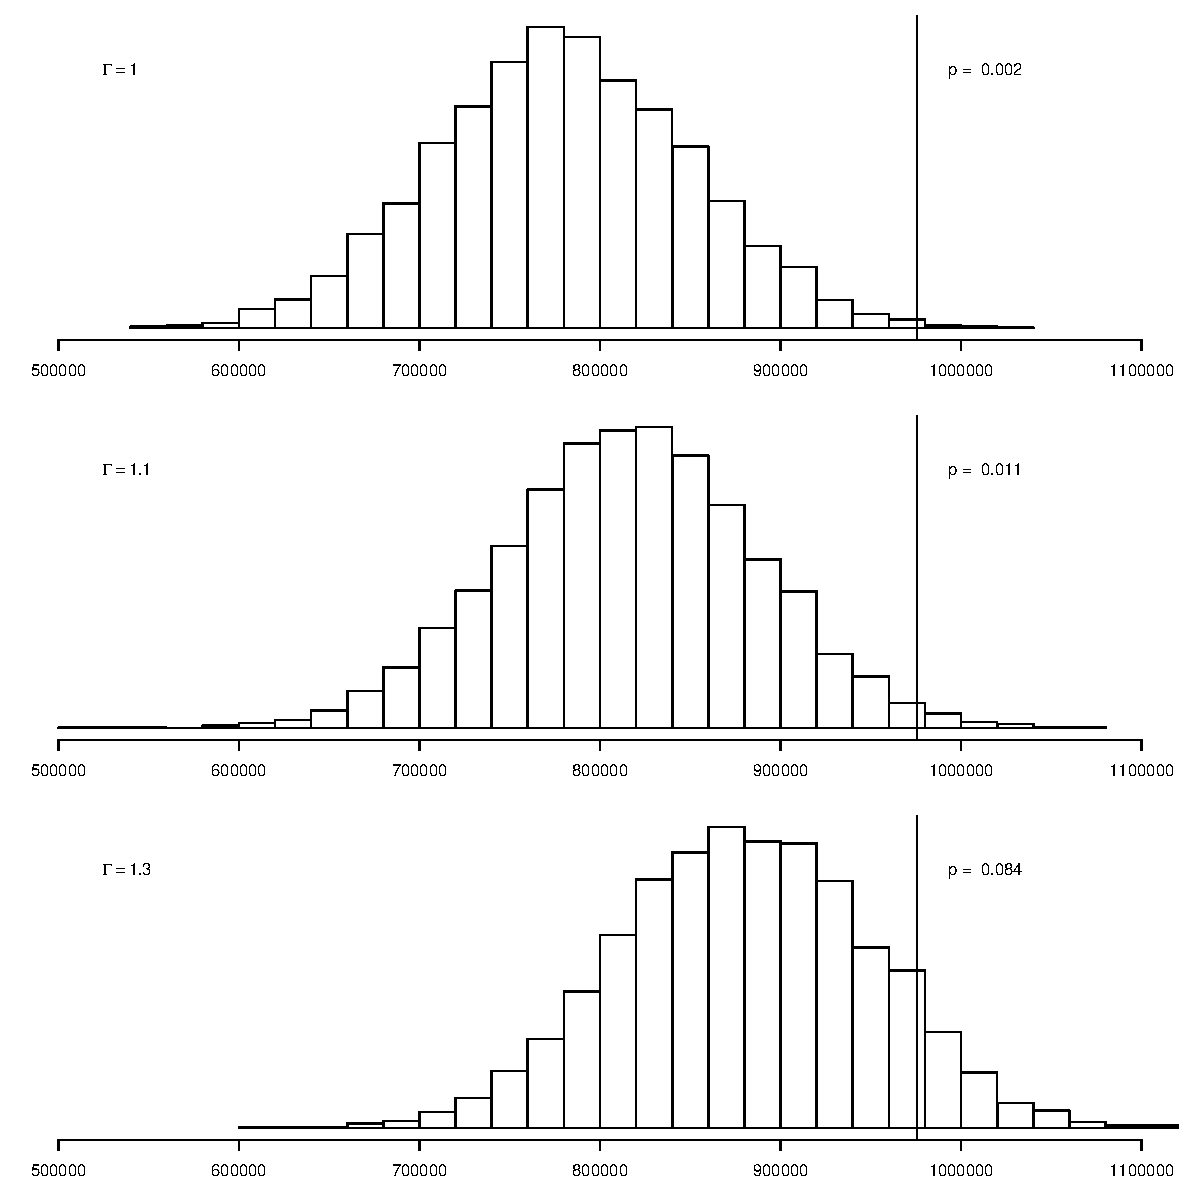
\includegraphics[width =  \textwidth]{figures/lalonde_hist_gamma.pdf}
\caption{The worst-case distributions of $T = \sumn S_i | \hat{\tau}_i |$ with $S_i$ IID Bernoulli$(\Gamma/(1+\Gamma))$, based on the matched LaLonde data.}\label{fg::lalonde_gamma}
\end{figure} 
 
 
 
 \begin{figure}
\centering
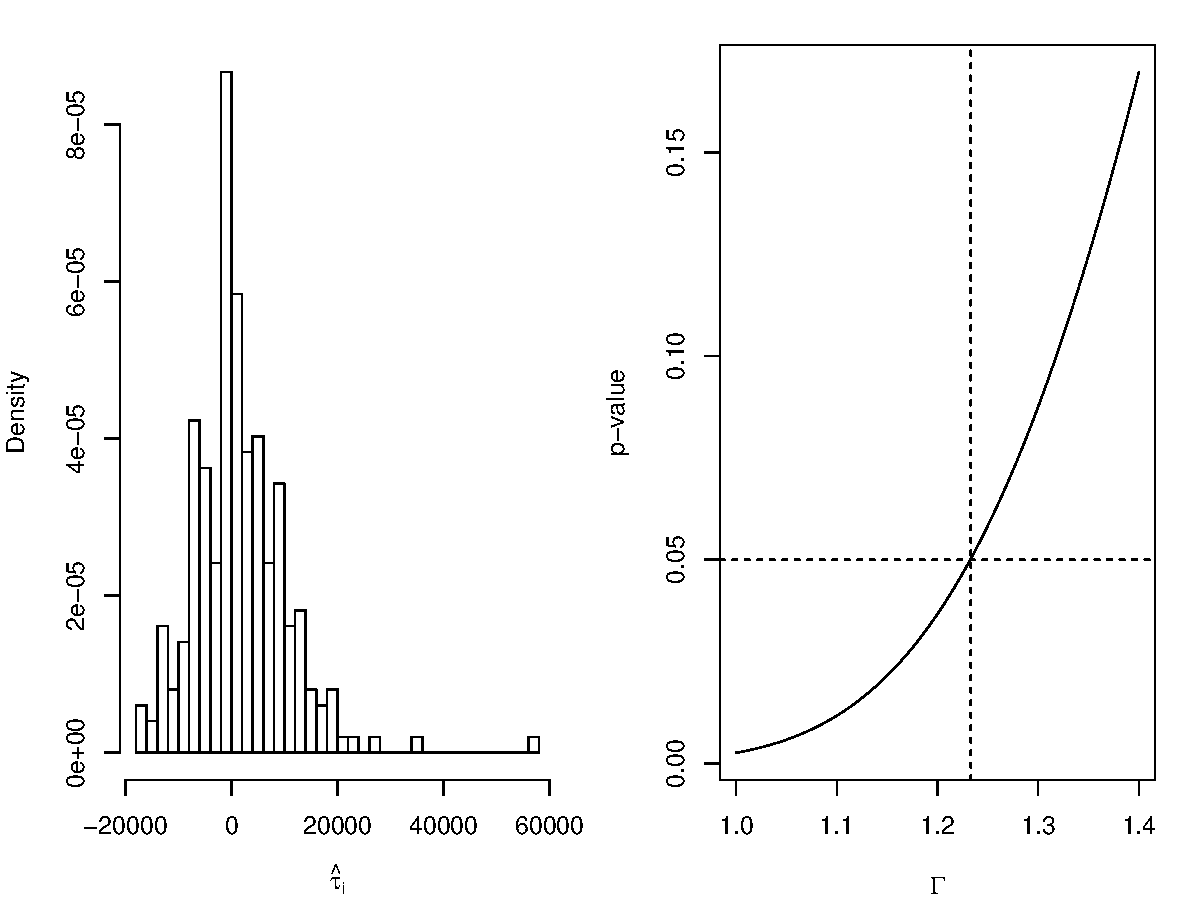
\includegraphics[width = \textwidth]{figures/lalonde_p_gamma.pdf}
\caption{$p$-value as a function of $\Gamma$, based on the matched LaLonde data.}\label{fg::p-gamma-lalonde}
\end{figure}



 
 
\subsection{Two examples from Rosenbaum's packages} 

 

 The \texttt{erpcp} dataset is from the \ri{R} package \texttt{sensitivitymw}. It contains $n=39$ matched pairs of a welder and a control, based on observed covariates age and smoking. The outcome is the DNA elution rate.  Figure \ref{fg::another2sensitivity}(a) shows the histogram of the within-pair differences of the outcomes and the $p$-value against $\Gamma$ based on the pair $t$-statistic. The following \ri{R} code generates Figure \ref{fig::erpcp}.
 
 
\begin{lstlisting}
par(mfrow = c(1, 2), mai = c(0.8, 0.8, 0.3, 0.3))
data(erpcp)
hist(erpcp[, 1] - erpcp[, 2], main = "erpcp",
     xlab = expression(hat(tau)[i]),
     freq = FALSE)

Gamma  = seq(1, 5, 0.005)
Pvalue = Gamma
for(i in 1:length(Gamma))
{
  Pvalue[i] = senmw(erpcp, gamma = Gamma[i], method = "t")$pval
}
gammastar = Gamma[which(Pvalue >= 0.05)[1]]
gammastar

plot(Pvalue ~ Gamma, type = "l", 
     xlab = expression(Gamma), 
     ylab = "p-value")
abline(h = 0.05, lty = 2)
abline(v = gammastar, lty = 2)
\end{lstlisting}


 The \texttt{lead250} dataset is from the \ri{R} package \texttt{sensitivitymw}. It contains $n=250$ matched pairs of a daily smoker and a control of nonsmoker, based on observed covariates gender, age, race education level, and household income from NHANES. The outcome is the blood lead level in $\mu g/l$. Figure \ref{fg::another2sensitivity}(b) shows the histogram of the within-pair differences of the outcomes and the $p$-value against $\Gamma$ based on the pair $t$-statistic. The following \ri{R} code generates Figure \ref{fig::ead250}.
 
 \begin{lstlisting}
par(mfrow = c(1, 2), mai = c(0.8, 0.8, 0.3, 0.3))
data(lead250)
hist(lead250[, 1] - lead250[, 2],
     main = "lead250",
     xlab = expression(hat(tau)[i]),
     freq = FALSE)

Gamma  = seq(1, 2.5, 0.001)
Pvalue = Gamma
for(i in 1:length(Gamma))
{
  Pvalue[i] = senmw(lead250, gamma = Gamma[i], method = "t")$pval
}
gammastar = Gamma[which(Pvalue >= 0.05)[1]]
gammastar

plot(Pvalue ~ Gamma, type = "l", 
     xlab = expression(Gamma), ylab = "p-value")
abline(h = 0.05, lty = 2)
abline(v = gammastar, lty = 2)
\end{lstlisting}


\begin{figure}
\centering 
\begin{subfigure}[b]{\textwidth}
                \centering
                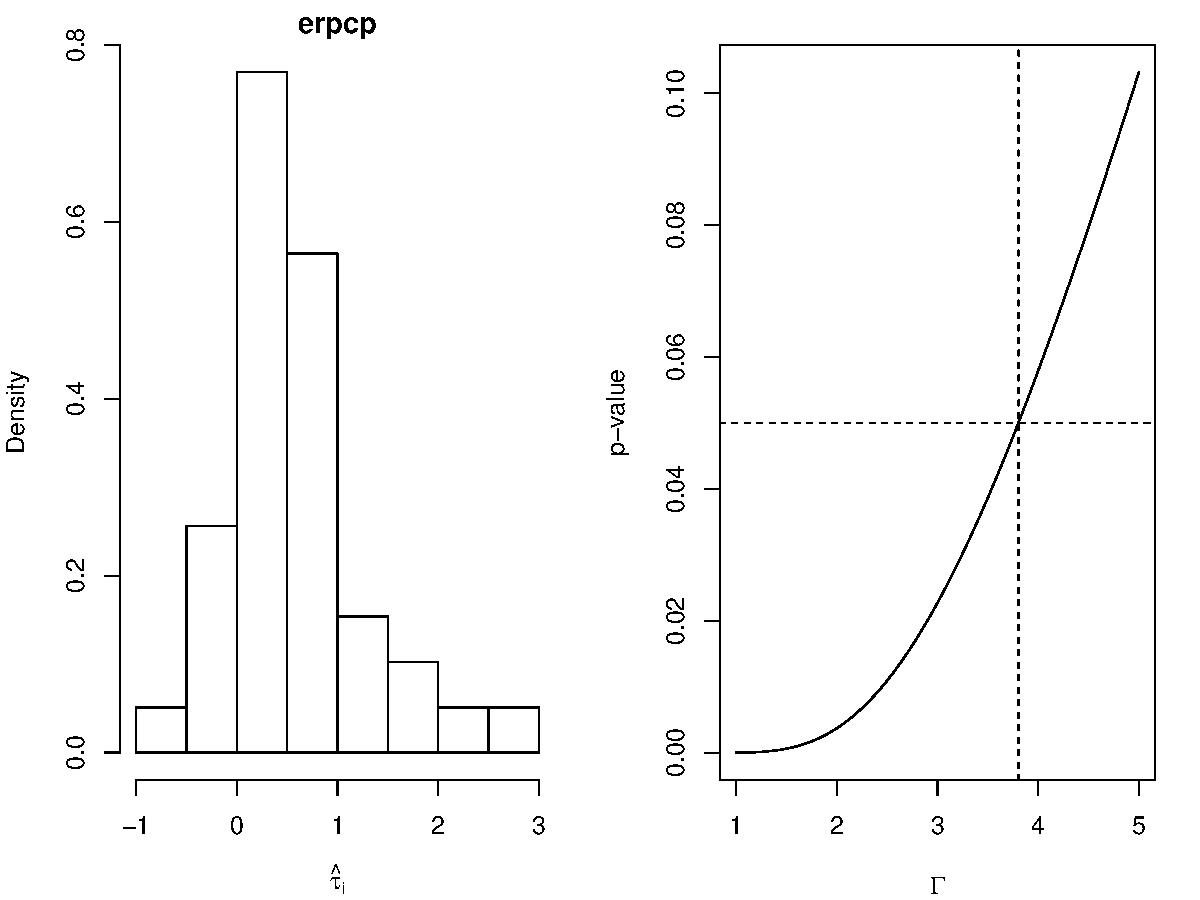
\includegraphics[width=\textwidth]{figures/erpcp_p_gamma.pdf}
                \caption{erpcp data}
                \label{fig::erpcp}
        \end{subfigure}%
        
        
        
        
        
        
\begin{subfigure}[b]{\textwidth}
                \centering
                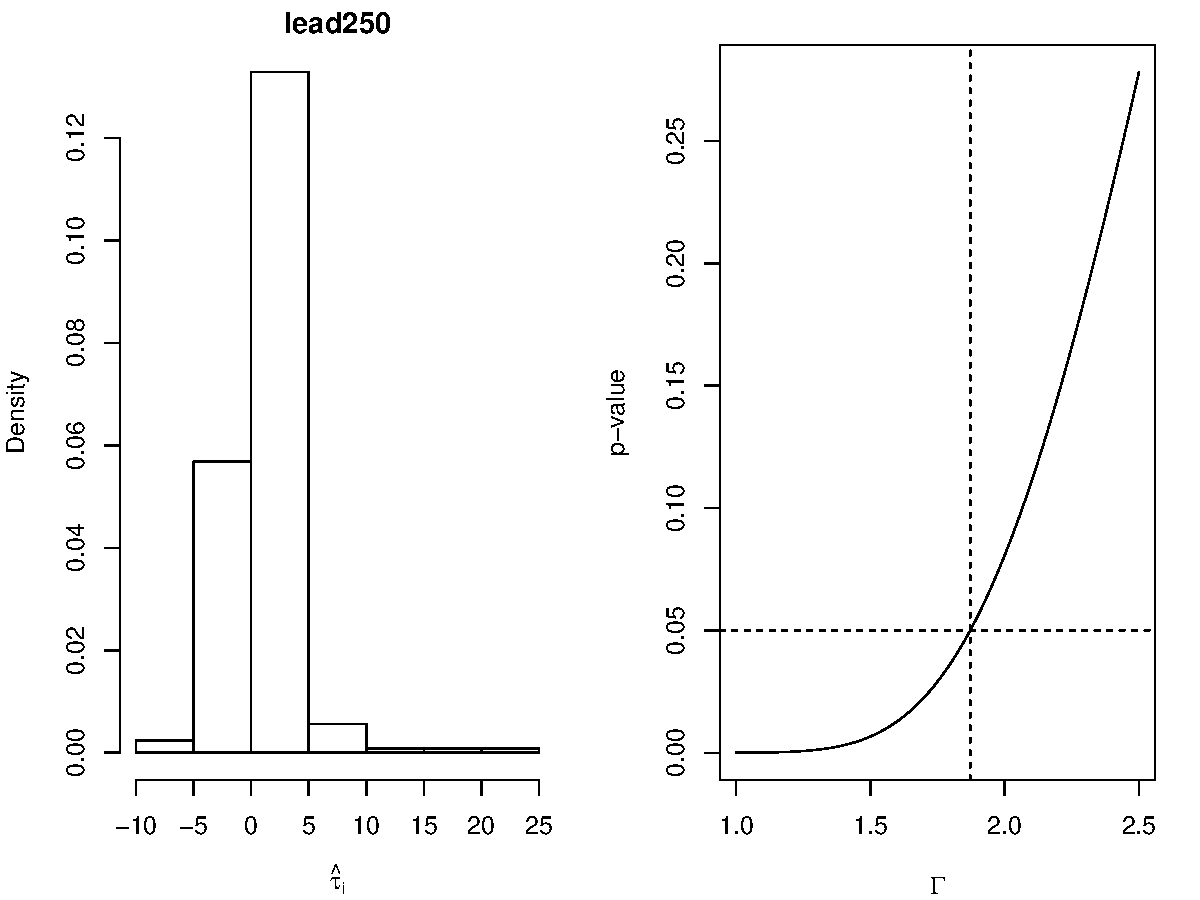
\includegraphics[width=\textwidth]{figures/lead250_p_gamma.pdf}
                \caption{ead250 data}
                \label{fig::ead250}
        \end{subfigure}%        
\caption{Two examples: histogram of the $\hat{\tau}_i$'s and $p$-value as a function of $\Gamma$}\label{fg::another2sensitivity}
\end{figure}


 
  

\section{Homework Problems}


\paragraph{A model for Assumption \ref{assume::rosenbaum-sensitivity}}\label{hw::rosenbaum-equivalent}

Assumption \ref{assume::rosenbaum-sensitivity} has the following equivalent form. 


\begin{assumption}
\label{assume::rosenbaum-equivalent}
The propensity score satisfies the following model
$$
\log \frac{  \pi_{ij} }{  1-\pi_{ij}  } = g(X_i) + \gamma U_{ij} ,\quad (i=1,\ldots, n; j=1,2)
$$
where $g(\cdot)$ is an unknown function and $U_{ij} \in [0, 1]$ is a a bounded unobserved covariate for unit $(i, j)$. 
\end{assumption}


Show that if Assumption \ref{assume::rosenbaum-equivalent} holds, then Assumption \ref{assume::rosenbaum-sensitivity} must hold with $\Gamma = e^\gamma$. 


Remark: \citet[][page 108]{rosenbaum2002design} also shows that if Assumption \ref{assume::rosenbaum-sensitivity} holds, then Assumption \ref{assume::rosenbaum-equivalent} must hold for some $U_{ij}$'s. Assumption \ref{assume::rosenbaum-equivalent} may be easier to interpret because $\gamma$ measures the log of the conditional odds ratio of $U$ on the treatment; see Chapter \ref{sec::logistic-regression} for the interpretation of the coefficients in the logistic regression. 



\paragraph{Application of Rosenbaum's approach}
Re-analyze Example \ref{eg::chan-bmi-ATE} using Rosenbaum's approach based on matching.



\paragraph{Recommended reading}


\citet{rosenbaum2015two} provides a tutorial for his two \ri{R} packages for sensitivity analysis with matched observational studies. 

